\documentclass{beamer}

\usepackage[portuguese]{babel}
\usepackage[utf8]{inputenc}
\usepackage{hyperref}
\usepackage[style=brazilian]{csquotes}
\usepackage{subcaption}
\usepackage{xcolor}
\usepackage{minted}
\usepackage{multicol}

\def\signed #1{{\leavevmode\unskip\nobreak\hfil\penalty50\hskip1em
  \hbox{}\nobreak\hfill #1%
  \parfillskip=0pt \finalhyphendemerits=0 \endgraf}}

\newsavebox\mybox
\newenvironment{aquote}[1]
  {\savebox\mybox{#1}\begin{quote}\openautoquote\hspace*{-.7ex}}
  {\unskip\closeautoquote\vspace*{1mm}\signed{\usebox\mybox}\end{quote}}

\usetheme{boxes}

\title{Obedecendo leis de trânsito com mapa topológico
\\\vspace{1.0cm}\centering
\includegraphics[height=0.35\textheight]{../imgs/duckieusp.png}
\vspace{-0.5cm}}
\date{}
\institute{\small MAC0318 - Introdução à Programação de Robôs Móveis\\~\\\scriptsize Instituto de
Matemática e Estatística (IME)\\Universidade de São Paulo (USP)}

\begin{document}

\begin{frame}
  \titlepage
\end{frame}

\begin{frame}
  \frametitle{Representação do mapa por grafo}

  Grafo $G=(V,E)$, onde:
  \vspace{0.5cm}

  \begin{itemize}
    \item Cada ``pedaço'' (\textit{tile}) de rua é um nó $v\in V$;
    \item Dois nós $u, v\in V$ estão conectados por uma aresta se é possível ir de $u$ até $v$ sem
      sair da rua.
  \end{itemize}
  \vspace{0.5cm}

  $G$ é uma representação ingênua. Como melhorar $G$ para respeitar as leis de trânsito?
\end{frame}

\begin{frame}
  \frametitle{Representação ingênua}

  \begin{figure}
    \centering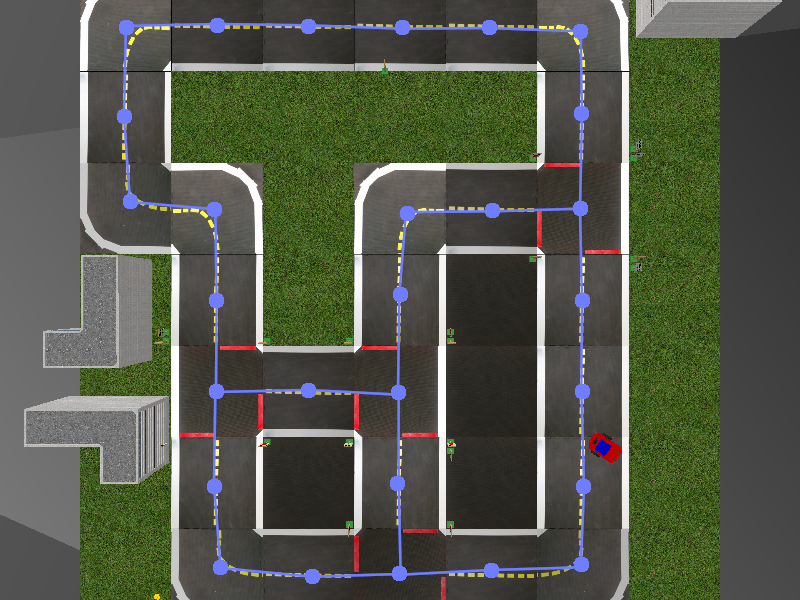
\includegraphics[height=0.7\textheight]{naive_rep.png}
  \end{figure}
\end{frame}

\begin{frame}
  \frametitle{Representação por único nó em intersecção}

  \begin{figure}
    \centering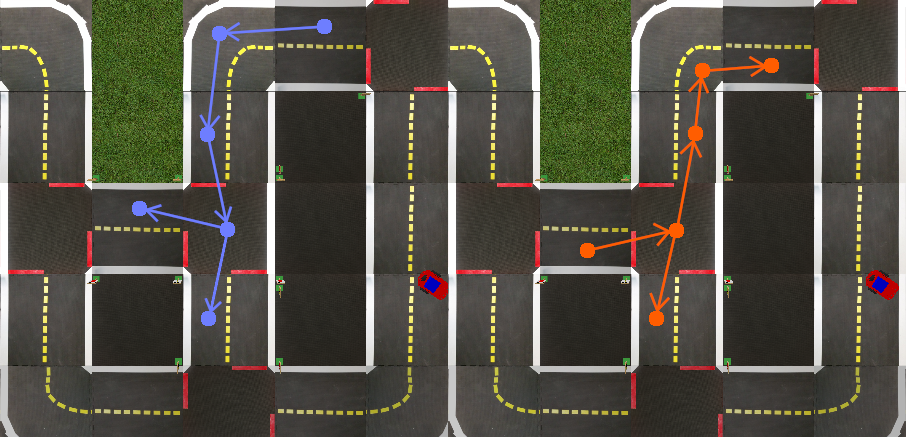
\includegraphics[width=\textwidth]{first_rep.png}
  \end{figure}
\end{frame}

\begin{frame}
  \frametitle{Representação por nó em cada faixa em intersecção}

  \begin{figure}
    \centering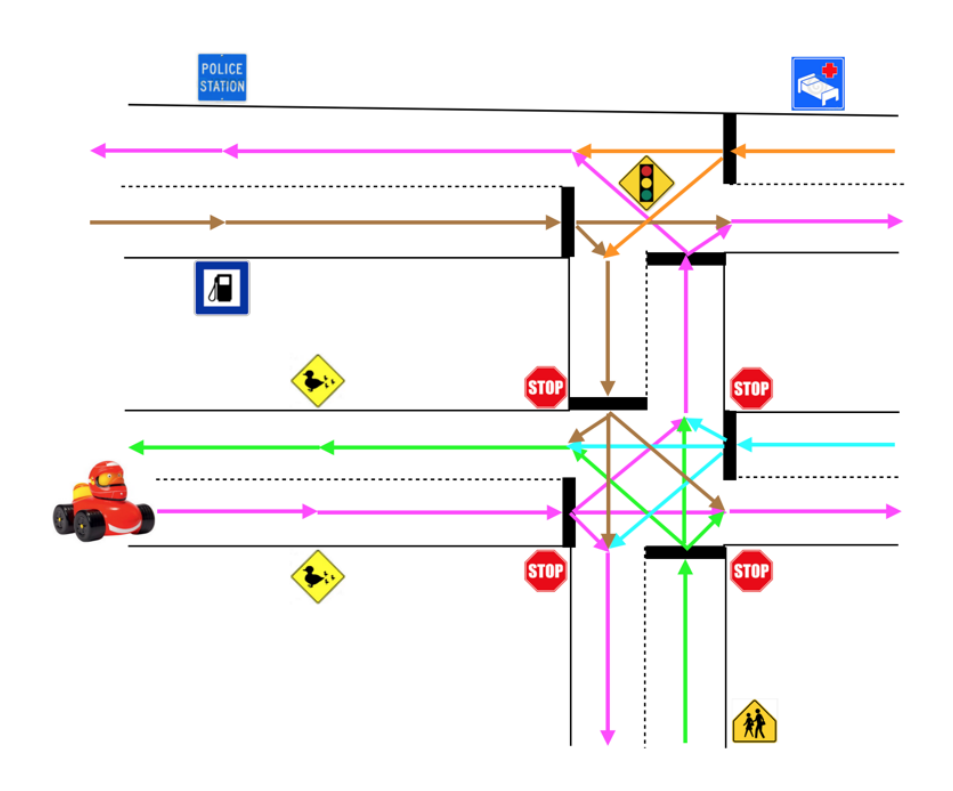
\includegraphics[height=0.7\textheight]{sec_rep.png}
    \caption*{\url{https://github.com/duckietown/lectures}}
  \end{figure}
\end{frame}

\begin{frame}[fragile]
  \frametitle{No código}

  \scriptsize
  \begin{multicols}{2}
  \begin{minted}{python}
class TopoGraph:
  def __init__(self, r):
    self._L = {}
    self._r = r

  def nodes(self):
    return list(self._L.keys())

  def edge(self, p, q):
    if self.invalid_tile(p, q):
      return False
    return q in self._L[p]

  def add_node(self, p):
    if p not in self._L:
      self._L[p] = {}

  def add_edge(self, p, q):
    self._L[p][q] = True
    self._L[q][p] = True

  def add_dir_edge(self, p, q):
    self._L[p][q] = True

  def bfs(self, p, q):
    p = self.closest_node(p)
    q = self.closest_node(q)
    Q = [p]
    V = {}
    Pa = {}
    while len(Q) != 0:
      n = Q.pop(0)
      if n == q:
        P = [q]
        while P[-1] != p:
          P.append(Pa[P[-1]])
        for i, u in enumerate(P):
          P[i] = u
        return P
      for c in self._L[n]:
        if c not in V:
          V[c] = True
          Pa[c] = n
          Q.append(c)
    return None

  \end{minted}
  \end{multicols}
\end{frame}

\begin{frame}
  \frametitle{Tarefa}

  Dado o grafo não direcionado da representação ``ingênua'', construa um grafo direcionado tal que
  o agente obedeça as seguintes regras de trânsito:
  \vspace{0.5cm}

  \begin{itemize}
    \item Ande sempre na faixa da direita;
    \item Retorno não é permitido em retas ou curvas;
    \item Sempre dirija ``para frente''.
  \end{itemize}
  \vspace{0.5cm}

  Arquivo esqueleto: \mintinline{bash}{assignments/topomap.py}
\end{frame}

\end{document}
